\chapter{2023/10/11}\label{20231011}

\section{Phase an group velocity
相速度和群速度}\label{phase-an-group-velocity-ux76f8ux901fux5ea6ux548cux7fa4ux901fux5ea6}

Phase velocity (相速度) \(v_p\) is the velocity of a certain phase that
travels: \[v_p = {\omega \over k}.\]

Group velocity (群速度) \(v_g\) is the velocity with which the envelope
of the wave (波包) propagates through space:
\[v_g = {\Delta \omega \over \Delta k}.\]

Energy is transmitted through \emph{group velocity}, not \emph{phase
velocity}.

\begin{quote}
For more reference, you can see:
\url{https://www.zhihu.com/question/29444240/answer/1833520606}.
\end{quote}

\section{Order of magnitude
数量级}\label{order-of-magnitude-ux6570ux91cfux7ea7}

For a number \(N\), we usually define its order of magnitude as follows:

Write the number in the form \[N =a \times 10 ^ b,\] in which
\[\dfrac{1}{\sqrt{10}} \leq a \leq \sqrt{10}, b \in \mathbb{Q},\] and
\(b\) is the \textbf{order of magnitude} of the number. For example:

\begin{center}
    \begin{tabular}{|c|c|c|}
        \hline
        $N$ & Expression in $N =a \times 10^b$ & Order of magnitude $b$ \\
        \hline
        $0.2$ & $2 \times 10^{-1}$ & $-1$ \\
        $1$ & $1 \times 10^{0}$ & $0$ \\
        $5$ & $0.5 \times 10^{1}$ & $1$ \\
        $6$ & $0.6 \times 10^{1}$ & $1$ \\
        $31$ & $3.1 \times 10^{1}$ & $1$ \\
        $32$ & $0.32 \times 10^{2}$ & $2$ \\
        $999$ & $0.999 \times 10^{3}$ & $3$ \\
        $1000$ & $1 \times 10^{3}$ & $3$ \\
        \hline
    \end{tabular}
    \captionof{table}{Order of Magnitude Examples}
\end{center}

Some constants in physics:

\begin{itemize}
\tightlist{}
\item
  Avogadro constant \(N_A = 6.02 \times 10^{23} \ \mathrm{mol^{-1}}\)
\item
  Reduced Planck constant
  \(\hbar = 1.054 \times 10^{-34} \ \mathrm{J \cdot s}\)
\item
  Speed of light \(c = 2.99792 \times 10^{8} \ \mathrm{m/s}\)
\item
  Boltzmann constant
  \(k_\mathrm{B} = 1.38 \times 10^{-23} \ \mathrm{J/K}\)
\item
  Fundamental charge \(e = 1.602 \times 10^{-19} \ \mathrm{C}\)
\item
  Universal gravitational constant
  \(G = 6.672 \times 10^{-11} \ \mathrm{N \cdot m^2/kg^2}\)
\end{itemize}

Note: This definition is not absolute. For example, some people tend to
use \(0.5 \leq a \leq 5\) or other criteria.

\section{A particular model
某个模型}\label{a-particular-model-ux67d0ux4e2aux6a21ux578b}

Below (Fig 8.1) is a container with two sides connected to each other by a small
hole.

To get the two sides to balance, we need to have \[\left\{
    \begin{aligned}
        & p_1 = p_2; \quad  &\text{pressure} &\\
        & T_1 = T_2; &\text{temperature} &\\
        & \mu_1 = \mu_2. &\text{chemical potential (化学势)} &
    \end{aligned}
\right.\]

\begin{center}
    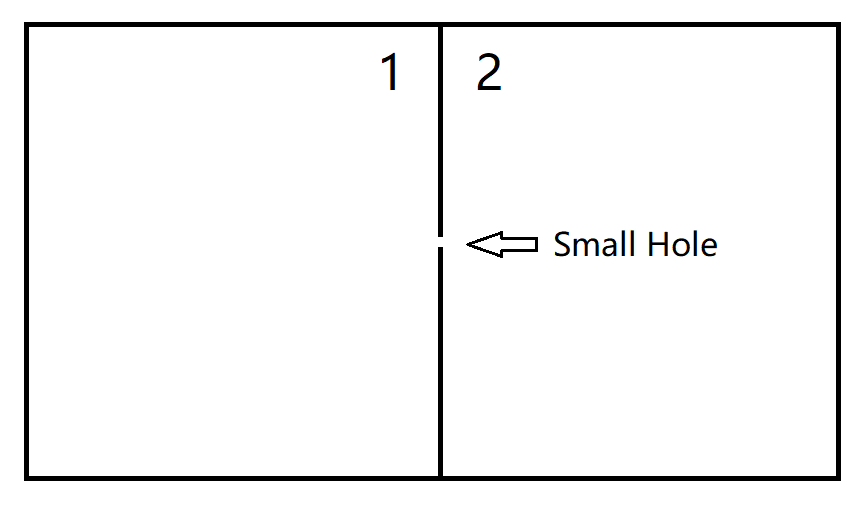
\includegraphics[height=100pt]{assets/Model_Two_sides.png}
    \captionof{figure}{A container with two sides}
\end{center}

Chemical potential \(\mu\) is defined as follows:

In a chemical system where there are \(n\) kinds of species (物种),
define \textbf{Gibbs free energy} (自由焓/吉布斯自由能) \[G=U-TS+pV\]
and the \textbf{chemical potential} (化学势) of species \(i\)
\[\mu_i = \left({\partial G \over \partial n_i}\right)_{T, p, n_j (j \neq i)}.\]

\section{About dimensional analysis and unit systems
关于量纲分析和单位制}\label{something-about-dimensional-analysis-and-unit-systems-ux4e00ux4e9bux5173ux4e8eux91cfux7eb2ux5206ux6790ux548cux5355ux4f4dux5236ux7684ux4e1cux897f}

Maxwell points out that:

\begin{enumerate}
\def\labelenumi{\arabic{enumi}.}
\item
  For a mechanical quantity (力学量), we only need three dimensions
  \(\mathrm{M, L, T}\) to form its unit and
\item
  Sometimes the dimensions of combined quantities (组合量的量纲) are
  more useful.
\end{enumerate}

There are two commonly-used unit systems in the world:

\begin{itemize}
\tightlist{}
\item \emph{Système
International} (SI) 国际单位制
\item Centimetre--gram--second system of units (CGS) 厘米--克--秒制
\end{itemize}

Let's look at a few examples.

\subsection*{(1) Coulomb's law
库仑定律}\label{coulombs-law-ux5e93ux4ed1ux5b9aux5f8b}

\[F = \left\{
\begin{aligned}
& \dfrac{q_1q_2}{4 \pi \varepsilon_0 r^2} & \text{(SI)} \\
& \dfrac{q_1q_2}{r^2} & \text{(CGS)}
\end {aligned}
\right.
\]

\subsection*{(2) Fine structure constant
精细结构常数}\label{fine-structure-constant-ux7cbeux7ec6ux7ed3ux6784ux5e38ux6570}

\[\alpha = \left\{
\begin{aligned}
& \dfrac{e^2}{4 \pi \varepsilon_0 \hbar c} & \text{(SI)} \\
& \dfrac{e^2}{\hbar c} & \text{(CGS)}
\end {aligned}
\right.
\approx {1 \over 137}.
\]

\emph{W. Pauli died in Room No.~137 in hospital. (地狱笑话了属于是)}

\subsection*{(3) Bohr radius
玻尔半径}\label{bohr-radius-ux73bbux5c14ux534aux5f84}

\[r_B = \left\{
\begin{aligned}
& \dfrac{4 \pi \varepsilon_0 \hbar^2}{m_e e^2} & \text{(SI)} \\
& \dfrac{\hbar^2}{m_ee^2} & \text{(CGS)}
\end {aligned}
\right.\]

\section{Planck units
普朗克单位}\label{planck-units-ux666eux6717ux514bux5355ux4f4d}

Planck units are a set of units that, by definition, are expressed using
these universal constants below, which, take the numeric value \(1\)
when expressed:

\begin{itemize}
\tightlist{}
\item
  the speed of light in vacuum \(c\)
\item
  the gravitational constant \(G\)
\item
  the reduced Planck constant \(\hbar\)
\item
  the Boltzmann constant \(k_\mathrm{B}\)
\end{itemize}

Typically we would use dimensional analysis to derive these units:
\[[c] = \mathrm{LT^{-1}};\]
\[[G] = {[F][r^2] \over [m_1m_2]} = \mathrm{\dfrac{ML}{T^2} \cdot L^2 \over M^2} = \mathrm{M^{-1}L^3T^{-2}};\]
\[[\hbar] = [E][t] = [mc^2][t] = \mathrm{ML^2T^{-1}};\]
\[[k_\mathrm{B}] = {[E] \over [T]} = {[mc^2] \over [T]} = \mathrm{ML^2T^{-2}\Theta^{-1}}.\]

\subsection*{(1) Planck length
普朗克长度}\label{planck-length-ux666eux6717ux514bux957fux5ea6}

\[\left[{G \hbar \over c^3}\right] = \mathrm{M^{-1}L^3T^{-2} \cdot ML^2T^{-1} \over (LT^{-1})^3} = \mathrm{L^2}.\]
\[l_P = \sqrt{G \hbar \over c^3}.\]

\subsection*{(2) Planck time
普朗克时间}\label{planck-time-ux666eux6717ux514bux65f6ux95f4}

\[t_P = {l_P \over c} = \sqrt{G \hbar \over c^5}.\]

\subsection*{(3) Planck mass
普朗克质量}\label{planck-mass-ux666eux6717ux514bux8d28ux91cf}

\[\left[{\hbar c \over G}\right]  = \mathrm{ML^2T^{-1} \cdot LT^{-1} \over M^{-1}L^3T^{-2}} = \mathrm{M^2}.\]
\[m_P = \sqrt{\hbar c\over G}.\]

\subsection*{(4) Planck temperature
普朗克温度}\label{planck-temperature-ux666eux6717ux514bux6e29ux5ea6}

\[\left[{\hbar c^5 \over Gk_\mathrm{B}^2}\right] = \mathrm{ML^2T^{-1} \cdot (LT^{-1})^5 \over M^{-1}L^3T^{-2} \cdot (ML^2T^{-2}\Theta^{-1})^2} = \mathrm{\Theta^2}.\]
\[T_P = \sqrt{\hbar c^5 \over Gk_\mathrm{B}^2}.\]

\subsection*{(5) Planck energy
普朗克能量}\label{planck-energy-ux666eux6717ux514bux80fdux91cf}

\[E_P = m_Pc^2 = \sqrt{\hbar c^5\over G}.\]

\subsection*{(6) Planck momentum
普朗克动量}\label{planck-momentum-ux666eux6717ux514bux52a8ux91cf}

\[p_P = m_Pc = \sqrt{\hbar c^3\over G}.\]

\subsection*{(7) Planck acceleration
普朗克加速度}\label{planck-acceleration-ux666eux6717ux514bux52a0ux901fux5ea6}

\[a_P = {c \over t_P} = \sqrt{c^7 \over \hbar G}.\]

\subsection*{(8) Planck force
普朗克力}\label{planck-force-ux666eux6717ux514bux529b}

\[F_P = m_P a_P = {c^4 \over G}.\]

Note that the Planck force can be \emph{hidden} in the Einstein
gravitational field equations: \[R_{\mu\nu} - {1 \over 2}g_{\mu\nu}R = 8 \pi \mathbf{G \over c^4}T_{\mu\nu} = {8 \pi \over \mathbf{F_P}} T_{\mu\nu}.\]

\emph{隐藏在引力方程中的力,被称为引力很合理吧?这恒河里!doge}

\subsection*{(9) Planck density
普朗克密度}\label{planck-density-ux666eux6717ux514bux5bc6ux5ea6}

\[\rho_P = {m_P \over {l_P}^3} = {c^5 \over \hbar G^2}.\]
